% Figure compendium: every size-quintile figure and the quintile summary table.
% Figures and tables are produced by notebooks/size_quintile_distributions.ipynb; re-run it before compiling.
\documentclass[11pt]{article}

\usepackage[margin=1in]{geometry}
\usepackage[T1]{fontenc}
\usepackage{newtxtext,newtxmath}   % Times, matching the figure typeface
\usepackage{amsmath}
\usepackage{graphicx}
\usepackage{booktabs}
\usepackage{float}
\usepackage[font=small,labelfont=bf,labelsep=period,justification=justified,singlelinecheck=false]{caption}
\usepackage[hidelinks]{hyperref}

\graphicspath{{../output/figures/quintiles/}}
\newcommand{\tablepath}{../output/tables}
\setlength{\parskip}{0.4em}

% Shared caption text
\newcommand{\quintnote}{Quintiles are formed each quarter from total assets at $t-1$.}
\newcommand{\recnote}{Shaded areas indicate NBER recessions.}
\newcommand{\bandnote}{Solid line: median bank; dark band: 25th--75th percentiles; light band: 10th--90th percentiles.}
\newcommand{\kdenote}{Gaussian kernel density, Silverman bandwidth. Horizontal axis spans the pooled 1st--99th percentiles.}
\newcommand{\histnote}{Histogram with no kernel smoothing; bar heights are bin counts divided by the full sample size and the bin width, so they share the vertical scale of the kernel densities. Horizontal axis spans the pooled 1st--99th percentiles.}
\newcommand{\source}{Source: FDIC Statistics on Depository Institutions; author's calculations.}

% Per-variable definitions
\newcommand{\defassets}{Percent change in each bank's total assets from the previous quarter; changes include mergers and acquisitions.}
\newcommand{\defequity}{Percentage-point change in each bank's equity capital to assets from the previous quarter.}
\newcommand{\defroa}{Percentage-point change in each bank's single-quarter ROA (annualized) from the previous quarter.}
\newcommand{\defnim}{Percentage-point change in each bank's single-quarter net interest margin (annualized) from the previous quarter.}
\newcommand{\defloans}{Percent change in each bank's net loans and leases from the previous quarter; includes mergers; banks with no loans in the previous quarter are excluded.}
\newcommand{\defdeposits}{Percent change in each bank's total deposits from the previous quarter; includes mergers.}
\newcommand{\defleverage}{Percentage-point change in each bank's Tier~1 leverage ratio from the previous quarter.}
\newcommand{\defnoncurrent}{Percentage-point change in each bank's noncurrent loans to loans from the previous quarter.}
\newcommand{\defchargeoffs}{Percentage-point change in each bank's single-quarter net charge-off rate (annualized) from the previous quarter.}
\newcommand{\defprovisions}{Percentage-point change in each bank's single-quarter provisions to assets (annualized) from the previous quarter.}
\newcommand{\defcostfunds}{Percentage-point change in each bank's single-quarter cost of funding earning assets (annualized) from the previous quarter.}

% \fan{file stem}{title}{definition}{optional cap sentence}
\newcommand{\fan}[4]{%
  \begin{figure}[H]
    \centering
    \includegraphics[width=\textwidth,height=0.78\textheight,keepaspectratio]{quintile_fan_#1_bare.pdf}
    \caption{#2, by size quintile. #3#4 \bandnote{} \quintnote{} \recnote{} \source}
    \label{fig:fan-#1}
  \end{figure}}

% \kdeq{file stem}{title}{definition}
\newcommand{\kdeq}[3]{%
  \begin{figure}[H]
    \centering
    \includegraphics[width=\textwidth]{quintile_kde_#1_bare.pdf}
    \caption{#2: pooled distribution by size quintile. \kdenote{} All quarters pooled. \quintnote{} #3 \source}
    \label{fig:kde-#1}
  \end{figure}}

% \kdecycle{file stem}{title}{definition}
\newcommand{\kdecycle}[3]{%
  \begin{figure}[H]
    \centering
    \includegraphics[width=\textwidth]{quintile_kde_cycle_#1_bare.pdf}
    \caption{#2: expansion versus recession quarters, within each size quintile. \kdenote{} Densities are estimated separately for expansion and recession quarters (quarters overlapping an NBER recession). \quintnote{} #3 \source}
    \label{fig:cycle-#1}
  \end{figure}}

% \ridge{file stem}{title}{definition}
\newcommand{\ridge}[3]{%
  \begin{figure}[H]
    \centering
    \includegraphics[width=\textwidth,height=0.78\textheight,keepaspectratio]{ridgeline_#1_bare.pdf}
    \caption{#2, by year, all banks. Gaussian kernel density of one-quarter changes, all quarters of each year pooled; each curve is scaled to a common peak height. Orange: years overlapping an NBER recession (2001, 2008, 2009, 2020). *2026 covers Q1--Q2 only. #3 \source}
    \label{fig:ridge-#1}
  \end{figure}}

% \disp{file stem}{title}{definition}
\newcommand{\disp}[3]{%
  \begin{figure}[H]
    \centering
    \includegraphics[width=\textwidth]{quintile_dispersion_#1_bare.pdf}
    \caption{#2: interquartile range (top) and Kelley skewness (bottom), by size quintile. Quantiles are computed each quarter within each size quintile, then smoothed with a centered four-quarter moving average. Kelley skewness $= (q_{90} + q_{10} - 2q_{50}) / (q_{90} - q_{10})$. \recnote{} #3 \source}
    \label{fig:disp-#1}
  \end{figure}}

% \histq{file stem}{title}{definition}
\newcommand{\histq}[3]{%
  \begin{figure}[H]
    \centering
    \includegraphics[width=\textwidth]{quintile_hist_#1_bare.pdf}
    \caption{#2: pooled empirical distribution by size quintile. \histnote{} 120 equal-width bins; all quarters pooled. \quintnote{} #3 \source}
    \label{fig:hist-#1}
  \end{figure}}

% \ridgehist{file stem}{title}{definition}
\newcommand{\ridgehist}[3]{%
  \begin{figure}[H]
    \centering
    \includegraphics[width=\textwidth,height=0.78\textheight,keepaspectratio]{ridgeline_hist_#1_bare.pdf}
    \caption{#2, by year, all banks: empirical histograms. \histnote{} 80 equal-width bins; all quarters of each year pooled; each histogram is scaled to a common peak height. Orange: years overlapping an NBER recession (2001, 2008, 2009, 2020). *2026 covers Q1--Q2 only. #3 \source}
    \label{fig:ridgehist-#1}
  \end{figure}}

\title{Distributions of Quarterly Changes by Bank Size Quintile:\\
       Figure Compendium, 1992--2026}
\author{William Rouse}
\date{\today}

\begin{document}
\maketitle

\tableofcontents
\clearpage

% ---------------------------------------------------------------------------
\section{Size cutoffs}

\begin{figure}[H]
  \centering
  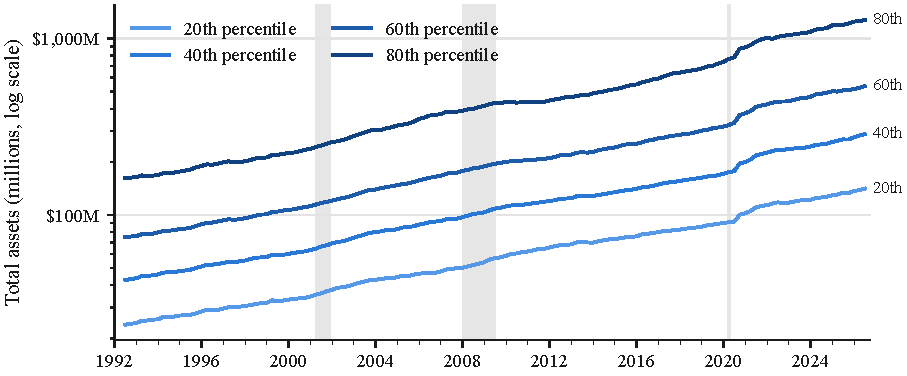
\includegraphics[width=\textwidth]{quintile_cutoffs_bare.pdf}
  \caption{Quintile cutoffs in dollars. Percentiles of total assets at the start of the quarter ($t-1$) that separate the five size quintiles, in nominal millions of dollars on a log scale. \recnote{} \source}
  \label{fig:cutoffs}
\end{figure}

\begin{table}[H]
  \centering
  \small
  \caption{Distribution of one-quarter changes by size quintile, expansion versus recession quarters. Median, interquartile range, and Kelley skewness are computed each quarter within each size quintile, then averaged over expansion and recession quarters.}
  \label{tab:summary}
  \input{\tablepath/quintile_summary.tex}
\end{table}

\clearpage
% ---------------------------------------------------------------------------
\section{Kernel densities by size quintile}

\kdeq{assets}{Change in total assets (\%)}{\defassets}
\kdeq{equity_ratio}{Change in equity capital to assets (pp)}{\defequity}
\kdeq{roa}{Change in return on assets (pp)}{\defroa}
\kdeq{nim}{Change in net interest margin (pp)}{\defnim}
\kdeq{loans}{Change in net loans and leases (\%)}{\defloans}
\kdeq{deposits}{Change in total deposits (\%)}{\defdeposits}
\kdeq{leverage}{Change in Tier~1 leverage ratio (pp)}{\defleverage}
\kdeq{noncurrent}{Change in noncurrent loans to loans (pp)}{\defnoncurrent}
\kdeq{chargeoffs}{Change in net charge-offs to loans (pp)}{\defchargeoffs}
\kdeq{provisions}{Change in provisions to assets (pp)}{\defprovisions}
\kdeq{cost_funds}{Change in cost of funding earning assets (pp)}{\defcostfunds}

\clearpage

\section{Ridgelines: the distribution year by year}

\ridge{assets}{Change in total assets (\%)}{\defassets}
\ridge{equity_ratio}{Change in equity capital to assets (pp)}{\defequity}
\ridge{roa}{Change in return on assets (pp)}{\defroa}
\ridge{nim}{Change in net interest margin (pp)}{\defnim}

\clearpage
% ---------------------------------------------------------------------------
\section{Empirical histograms by size quintile}

Unsmoothed counterparts of the kernel densities in Section~2. Each quintile's distribution is drawn as a step histogram on common equal-width bins over the same window, with no bandwidth choice involved. Mass points the kernel spreads out (for example, the exact zeros in charge-offs and provisions from banks with none in either quarter) appear here as single tall bins.

\histq{assets}{Change in total assets (\%)}{\defassets}
\histq{equity_ratio}{Change in equity capital to assets (pp)}{\defequity}
\histq{roa}{Change in return on assets (pp)}{\defroa}
\histq{nim}{Change in net interest margin (pp)}{\defnim}
\histq{loans}{Change in net loans and leases (\%)}{\defloans}
\histq{deposits}{Change in total deposits (\%)}{\defdeposits}
\histq{leverage}{Change in Tier~1 leverage ratio (pp)}{\defleverage}
\histq{noncurrent}{Change in noncurrent loans to loans (pp)}{\defnoncurrent}
\histq{chargeoffs}{Change in net charge-offs to loans (pp)}{\defchargeoffs}
\histq{provisions}{Change in provisions to assets (pp)}{\defprovisions}
\histq{cost_funds}{Change in cost of funding earning assets (pp)}{\defcostfunds}

\clearpage

\section{Empirical ridgelines: the distribution year by year}

Unsmoothed counterparts of the ridgelines in Section~3: one histogram per calendar year, all banks.

\ridgehist{assets}{Change in total assets (\%)}{\defassets}
\ridgehist{equity_ratio}{Change in equity capital to assets (pp)}{\defequity}
\ridgehist{roa}{Change in return on assets (pp)}{\defroa}
\ridgehist{nim}{Change in net interest margin (pp)}{\defnim}

\end{document}
